\documentclass[journal]{IEEEtran}

\usepackage[T1]{fontenc}  
\usepackage[utf8]{inputenc}  
\usepackage[portuguese]{babel}
\usepackage{graphicx}
\usepackage{subfigure}
\usepackage{enumerate}
\usepackage{ae}
\usepackage{color}
\usepackage{epstopdf}
\usepackage{placeins}


\hyphenation{op-tical net-works semi-conduc-tor}

\begin{document}

\title{Introdução ao Processamento de Imagens}

\author{Victória Goularte - 12/0137691}

\markboth{Universidade de Brasília - UnB}
{Shell \MakeLowercase{\textit{et al.}}: Bare Demo of IEEEtran.cls for IEEE Journals}

\maketitle

\begin{abstract}
No trabalho são aplicadas operações consideradas de médio nível no processamento digital de imagens. São as operações morfológicas, de segmanetação e codificação de vídeo.
\end{abstract}

\section{Introdução}

\IEEEPARstart{F}{ace Swapping} é uma técnica de processamento de imagens que digitalmente envolve troca de rostos de dois ou mais sujeitos retratados em uma determinada fotografia. Uma variação conhecida da prática é facebombing , uma técnica similar que envolve tomar uma face em um grupo e aplicá-lo a todas as faces da foto. A prática aumentou radicalmente em popularidade em 2015, quando vários aplicativos automatizados foram criados para trocar instantaneamente os rostos na fotografia e vídeo.


	A origem exata da troca de rosto é desconhecido, mas sua popularidade como um método de criação de imagens exploráveis ​​remonta ao início do Photoshop. 


\section{Metodologia}
O trabalho foi dividido em algumas partes, que serão tratadas separadamente a seguir:\newline

\subsection*{Parte I}
Primeiramente foram lidas duas imagens. Uma que será retirada as regiões de interesse como: olhos, nariz e boca; e outra que servirá de rosto base para a inserção dessas regiões.

As imagem foram redimensionadas para 250x250 pixels para que pussuam as mesmas dimenções.

\begin{figure}[h]
\centering
\subfigure[Imagem base]{
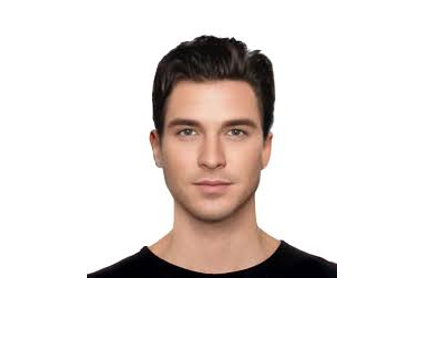
\includegraphics[scale=0.3]{imagem1.jpg}}
\subfigure[Imagem recorte\label{red2}]{
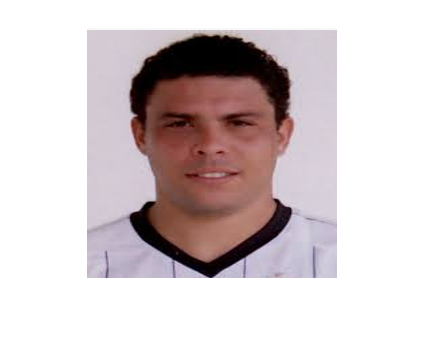
\includegraphics[scale=0.3]{imagem2.jpg}}
\end{figure}

\newline

\subsection*{Parte II}
Logo em seguida, foram detectadas as regiões de interesse (olhos, nariz e boca) e recortadas da imagem.\\


\begin{figure}[h]
\centering
\subfigure[Imagem detecção]{
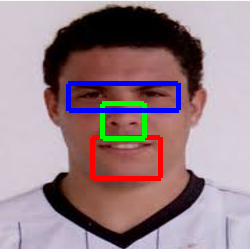
\includegraphics[scale=0.3]{deteccao.png}}
\subfigure[\label{red2}]{
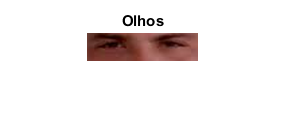
\includegraphics[scale=0.5]{olhos.png}}
\subfigure[\label{red2}]{
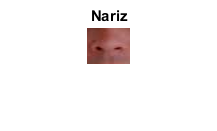
\includegraphics[scale=0.5]{nariz.png}}
\subfigure[\label{red2}]{
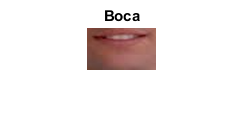
\includegraphics[scale=0.5]{boca.png}}
\end{figure}
\floatBarrier	

\subsection*{Parte III}

Posteriormente, realizou-se a detecção das posições locais de recursos e limites nos rostos detectados.

Para isso foi utilizada a função do MATLAB \textit{convhull}, função que retorna o casco convexo de um conjunto de pontos no espaço 2D ou 3D. Nesse caso, retorna o casco limitado pelos olhos, boca e nariz obtidos anteriormente. E também foi utilizada a função de detecção de bordas \textit{Sobel}.
\begin{figure}[h]
\centering
\subfigure[Convex-hull e borda]{
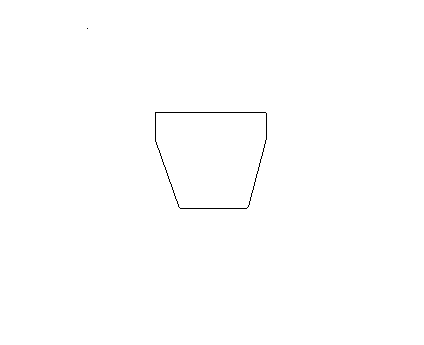
\includegraphics[scale=0.3]{borda.png}}
\subfigure[Resultado \label{red2}]{
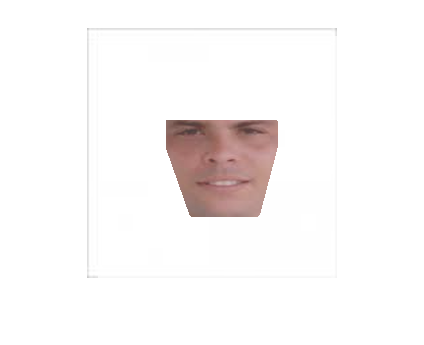
\includegraphics[scale=0.3]{covex_hull.png}}
\end{figure}

\subsection{Parte IV}

A partir das características foram criados pontos de destino para o mapeamento de um rosto para o outro. Obtendo assim a possição exata do rosto base.
Comparacao de posição:

\begin{figure}[h]
\centering
\subfigure[Posição original]{
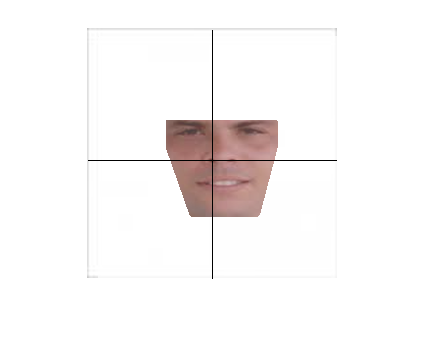
\includegraphics[scale=0.3]{posicao_original.png}}
\subfigure[Nova posicao \label{red2}]{
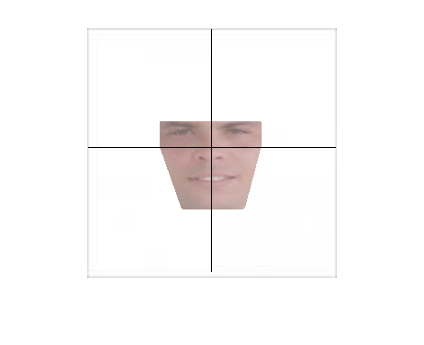
\includegraphics[scale=0.3]{nova_posicao.png}}
\end{figure}



\subsubsection*{2.1}
A imagem foi binarizada como na primeira parte, onde as células são pretas e o fundo é branco

\begin{figure}[!htb]
	\centering
	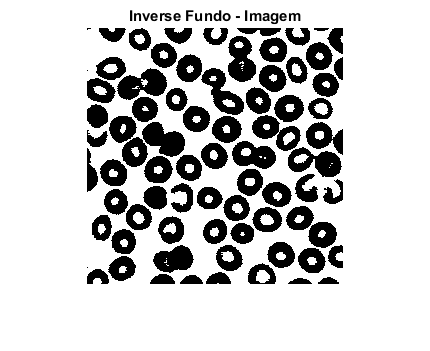
\includegraphics[scale=0.5]{2-1.png}
	\caption{Imagem binarizada}
	\label{Original}
\end{figure}

\subsubsection*{2.2}
A função \textit{bwareopen} para preencher espaços desconectados\newline
\\ 

\begin{figure}[!htb]
	\centering
	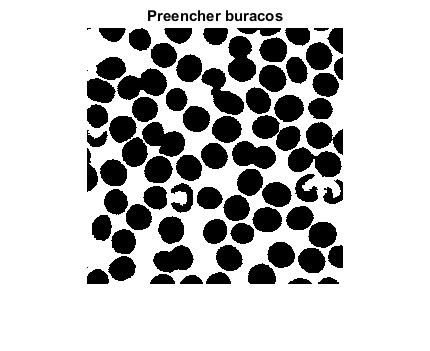
\includegraphics[scale=0.5]{2-buracos.png}
	\caption{Imagem Buracos Preenchidos}
	\label{Original}
\end{figure}

\subsubsection*{2.3}
A distância foi calculada através da função \textit{bwdist} usando o complemento da imagem

\begin{figure}[!htb]
	\centering
	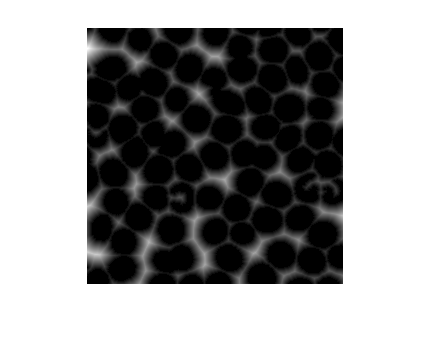
\includegraphics[scale=0.5]{2distancia.png}
	\caption{Distância}
	\label{Original}
\end{figure}

\subsubsection*{2.4}
Por fim, essa imagem foi segmentada, a fim de dividir os objetos que a compõe\newline
\\ 

\begin{figure}[!htb]
	\centering
	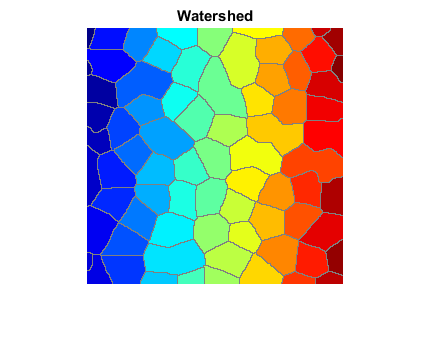
\includegraphics[scale=0.5]{2-wathershed.png}
	\caption{Distância}
	\label{Original}
\end{figure}

Nota-se que a imagem não foi perfeitamente segmentada, ou seja, os objetos não foram todos perfeitamente divididos, já que na binarização algumas células se mantiveram unidas, mesmo aplicando outras operações morfológicas para separá-las.

\subsection{Parte III}
Na terceira e última parte, foi feita uma função ler\_yuv que recebe como parâmetros um arquivo YUV, sua resolução, o formato (4:2:0) e o número do quadro a ser lido, e seu retorno é a imagem desse quadro.

A seguir são feitas novas funções que estimam o movimento (DPCM) entre um quadro e outro, recuperados a partir da função já citada. Essas funções foram feitas a partir do algoritmo de Block Matching para estimação de movimento.

As funções implementadas no projeto foram:

\begin{itemize}
	\item LogSearch;
	\item Motion\_Est;
	\item reconstruct;
	\item FullSearch;
	\item Bidirectional\_ME.
\end{itemize}

Resultados obtidos com blocos de tamanho 8x8 a partir dos frames 100 e 150 do arquivo '\textit{foreman.yuv}':

\begin{figure}[h]
\centering
\subfigure[Vetores de movimento]{
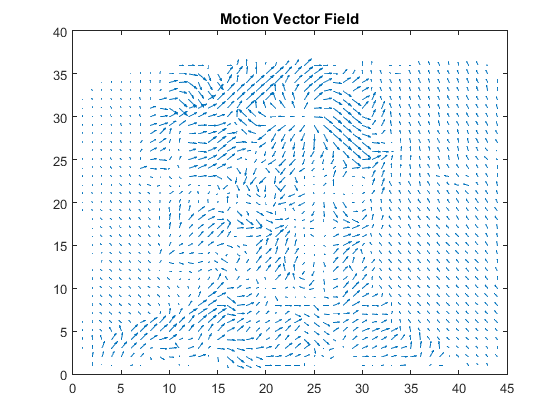
\includegraphics[scale=0.25]{3-1-motionvec.png}}
\subfigure[1º Frame]{
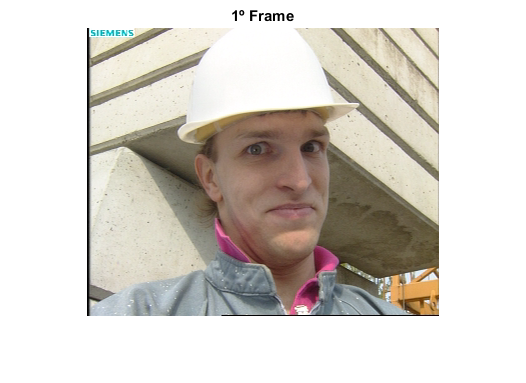
\includegraphics[scale=0.25]{3-1-f1.png}}
\subfigure[2º Frame\label{red2}]{
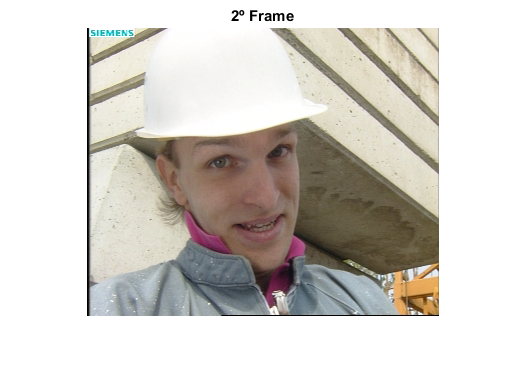
\includegraphics[scale=0.25]{3-1-f2.png}}
\subfigure[Resultado\label{red2}]{
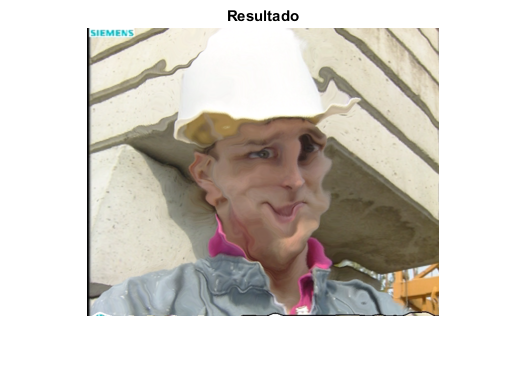
\includegraphics[scale=0.25]{3-1-resultado.png}}
\subfigure[SPRN]{
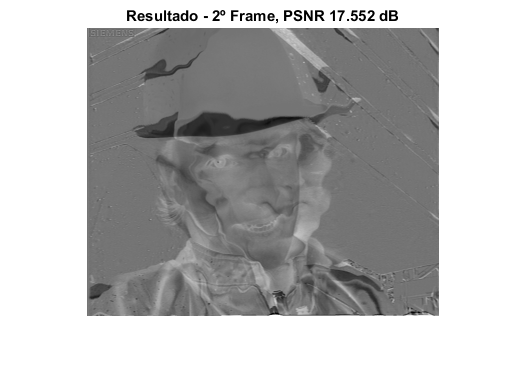
\includegraphics[scale=0.25]{3-1-psnr.png}}
\end{figure}

Resultados obtidos com blocos de tamanho 4x4 a partir dos frames 100 e 150 do arquivo '\textit{foreman.yuv}':

\begin{figure}[h]
\centering
\subfigure[Vetores de movimento]{
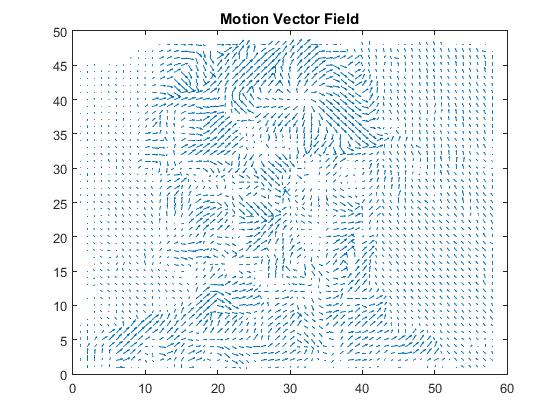
\includegraphics[scale=0.25]{3-2-motionvec.png}}
\subfigure[1º Frame]{
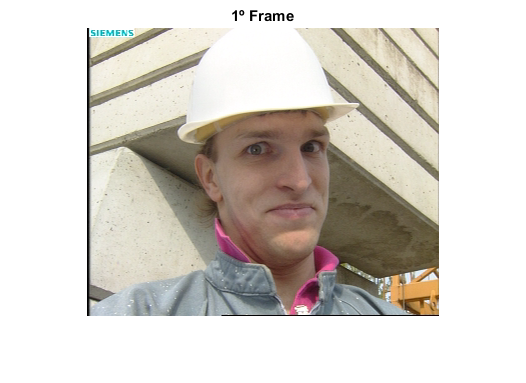
\includegraphics[scale=0.25]{3-2-f1.png}}
\subfigure[2º Frame\label{red2}]{
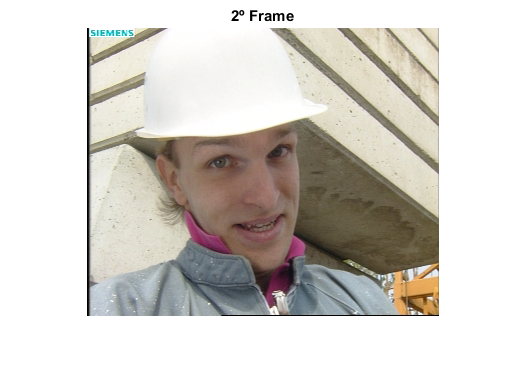
\includegraphics[scale=0.25]{3-2-f2.png}}
\subfigure[Resultado\label{red2}]{
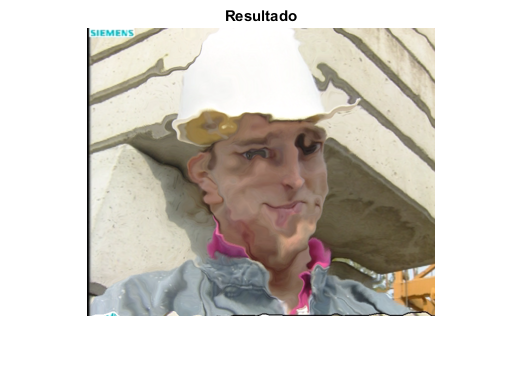
\includegraphics[scale=0.25]{3-2-resultado.png}}
\subfigure[SPRN]{
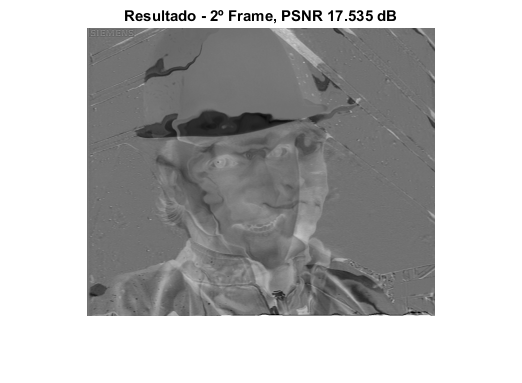
\includegraphics[scale=0.25]{3-2-psnr.png}}
\end{figure}

É notório como quanto menor o bloco, melhor a estimativa do movimento.

\ifCLASSOPTIONcaptionsoff
  \newpage
\fi

\section{Conclusão}
A partir dos resultados obtidos, na primeira parte nota-se que a definição da morfologia bottom-hat, que destaca objetos escuros sobre um fundo claro, aplicando fechamento na imagem para obter o fundo e posteriormente subtraindo a imagem por esse fundo encontrado é afirmada. Na segunda parte, aplicando segmentação seguindo os passos instruídos, tem-se o subdivisão da imagem em objetos ou regiões como era esperado, podendo servir para diversas aplicações que necessitam dos objetos isolados. E, por fim, um vídeo YUV é lido a partir dos parâmetros solicitados, e são recuperados frames especificos nessa função e aplica-se o algoritmo de Block Matching para estimação do movimento que foi claramente aplicado.

\begin{thebibliography}{1}

\bibitem{IEEEhowto:kopka}

http://scholar.harvard.edu/stanleychan/software/subpixel-motion-estimation-without-interpolation

Materiais da disciplina

\end{thebibliography}




\end{document}


